% Template for ICASSP-2010 paper; to be used with:
%          mlspconf.sty  - ICASSP/ICIP LaTeX style file adapted for MLSP, and
%          IEEEbib.bst - IEEE bibliography style file.
% --------------------------------------------------------------------------
\documentclass{article}
\usepackage{amsmath,graphicx,02460}



\toappear{02456 Deep Learning, DTU Compute, Fall 2017}


% Example definitions.
% --------------------
\def\x{{\mathbf x}}
\def\L{{\cal L}}

% Title.
% ------
\title{Raman spectroscopy deconvolution using stacked Auto-Encoders with non-negativity constraints}
%
% Single address.
% ---------------
\name{Jacob S. Larsen, Flavia D. Frumosu, Jakob Thrane, Maximillian F. Vording, Tommy S. Alstrøm \thanks{Thanks to XYZ agency for funding.}}
\address{Department of Applied Mathematics and Computer Science, Technical University of Denmark}
%
% For example:
% ------------
%\address{School\\
%	Department\\
%	Address}
%
% Two addresses (uncomment and modify for two-address case).
% ----------------------------------------------------------
%\twoauthors
%  {A. Author-one, B. Author-two\sthanks{Thanks to XYZ agency for funding.}}
%	{School A-B\\
%	Department A-B\\
%	Address A-B}
%  {C. Author-three, D. Author-four\sthanks{The fourth author performed the work
%	while at ...}}
%	{School C-D\\
%	Department C-D\\
%	Address C-D}
%
\begin{document}
%\ninept
%

\maketitle
%
\begin{abstract}

\end{abstract}
%
\begin{keywords}
One, two, three, four, five
\end{keywords}
%
\section{Introduction}
\label{sec:intro}

Raman scattering is a technique used to detect and identify molecules using the interaction of photons. It is a technique that is commonly used in chemistry and physics for detecting molecules by observing their vibrational and rotational modes. This is completed with the use of laser light. The photon excites the sample which causes scattering, meaning the photon has a change in energy over a short time period. This energy-change is reflected as a shift in frequency, also called a stokes shift, and by analysing the spectrum the molecules and combination of molecules can be identified. 

Surface-enhanced Raman Scattering (SERS) is an enhancement of Raman Scattering, that uses surfaces such as metal or nanostructures to absorb molecules. This enables the identification of single molecules.  For instance, noble metal nanostructures can concentrate light which greatly enhances the electromagnetic field near the nanostructure. These areas become so called "hot spots" that amplify weak Raman scattering signals which may not have been possible to detect with regular Raman scattering. The placement and design of these nanostructers with high SERS preformance is beyond the scope of this work, however additional information can be found in \cite{Wei2013} and references herein.

Complex mixtures in spectra.

NMF/MCR for source seperation and mixture classification.

Computational heavy for increased resolution of Raman spectras.

Sparse autoencoder

\section{Prior work}
\label{sec:prior}



Primary reference \cite{Hosseini-Asl2016}

\section{Methods}
\label{sec:methods}

This work seeks to compare traditional and proven methods for SERS analysis, i.e. curve resolution, such as NMF to denoising autoencoders with non-negativity constraints. 
\textbf{Add how NMF/MCR is used in raman spectroscopy.}

\subsection{Non-negative matrix factorization}

Non-negative matrix factorization (NMF) consists of factorizing a original matrix $V$, with only positive elements, into two positive matrices $W$ and $H$. \cite{Seung1999}


\begin{equation}
V \approx W \times H
\end{equation}

Where columns of $W$ are considered basis vectors, and each column in $H$ is considered an encoding with a one-to-one relationship with the columns of $V$. So for instance, a matrix V of size $n \times m$ can be factorized into a matrix $W$ of size $n \times k$ and a matrix $H$ of size $k \times m$, where $k$ is the number of components. Approaching the intuitive point of view, $W$ and $H$ can be seen as components that combined approximate the original signal $V$.

An iterative algorithm is considered for NMF, which shares similar monotonic convergence as the EM algorithm. \cite{Dempster1977}. Moreover, the rules of update preserve non-negativity of $W$ and $H$. The algorithm approaches the problem by initialization of $W$ and $H$ as non-negative, and then update the values in $W$ and $H$ until local maximima is obtained and both matrixes are considered stable. The rules of multiplicative update can be defined as:

\begin{equation}
H^{n+1} \leftarrow H^{n} \frac{(W^n)^TV}{(W^n)^TW^nH^n}
\end{equation}
and 
\begin{equation}
W^{n+1} \leftarrow W^{n} \frac{V(H^{n+1})^T}{WH^{n+1}(H^{n+1})^T}
\end{equation}

This however leads to an optimization that is convex for $W$ and $H$ which can require many iterations and poor local minima. For this problem, alternating least squares (ALS) is commonly used. This consists by alternating the optimization between $W$ and $H$, e.g. one interation consists of 1) keeping $H$ fixed while solving for $W$, and 2) keeping $W$ fixed while solving for $H$. Further details can be found in  \cite{Langville2014} and references herein. This is, for the remainder for this work, defined as NMF-ALS.

\subsection{Sparse auto-encoder with non-negativity constraint}

Reconstruction of input vector through unsupervised learning. Parametric deterministic mapping \cite{Vincent}

\begin{equation}
y = f(x) = \mathbf{W}x + \mathbf{b}
\end{equation}

Where $x$ is the input vector and $\mathbf{W}$ is a mtrix of weights and $\mathbf{b}$ is a bias vector. $y$ is the latent representation that is reconstructed in input space by 

\begin{equation}
z = g(y) = \mathbf{W'}x + \mathbf{b'}
\end{equation}
Primary reference implementation. Describe the constraint and the training architecture

\section{Setup}
\label{sec:setup}


Dataset origin, description of wavenumbers, raman map size. Definitions for the rest of the paper.

architecture drawing with stacked training and softmax/sigmoid layer.

MNIST verification

\section{Results}
\label{sec:results}

Training and test data. 

Encodings and basis vectors

\begin{figure}
  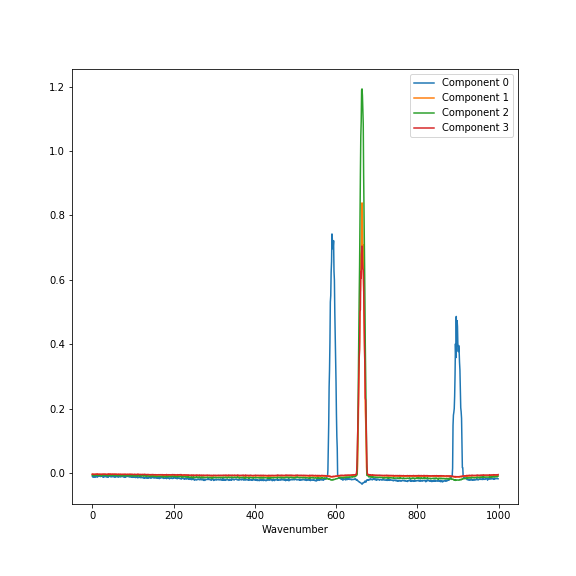
\includegraphics[width=0.5\textwidth]{figures/raman_sim_3_encode_layer_1_finetune_13.png}
\end{figure}


\begin{figure}
  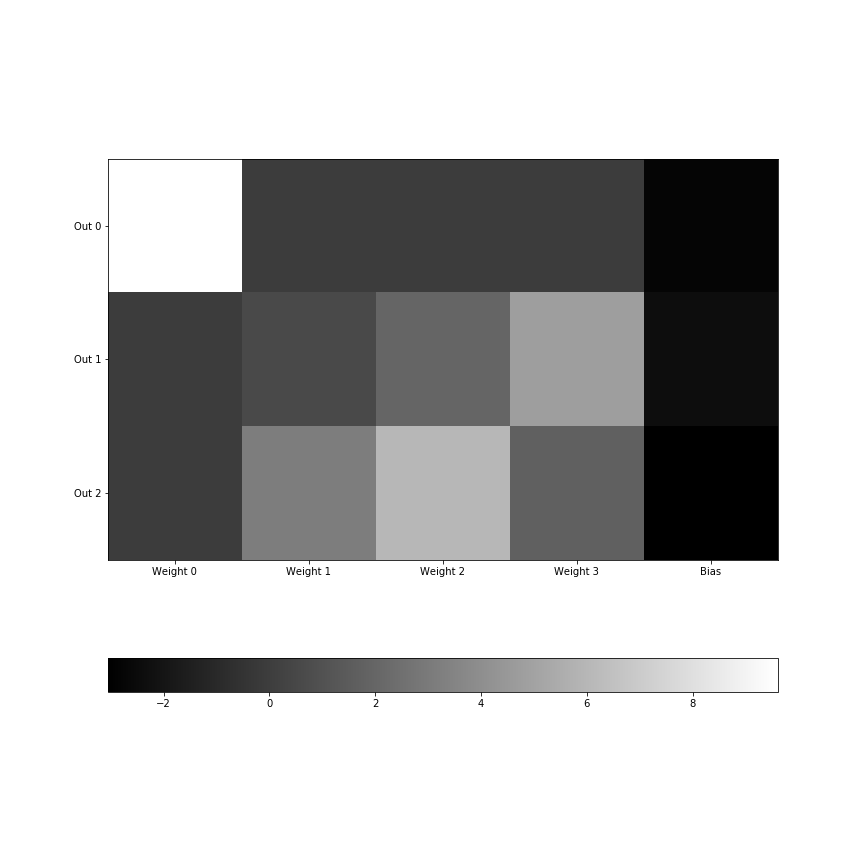
\includegraphics[width=0.23\textwidth]{figures/raman_sim_3_encode_layer_2_finetune_13.png}
  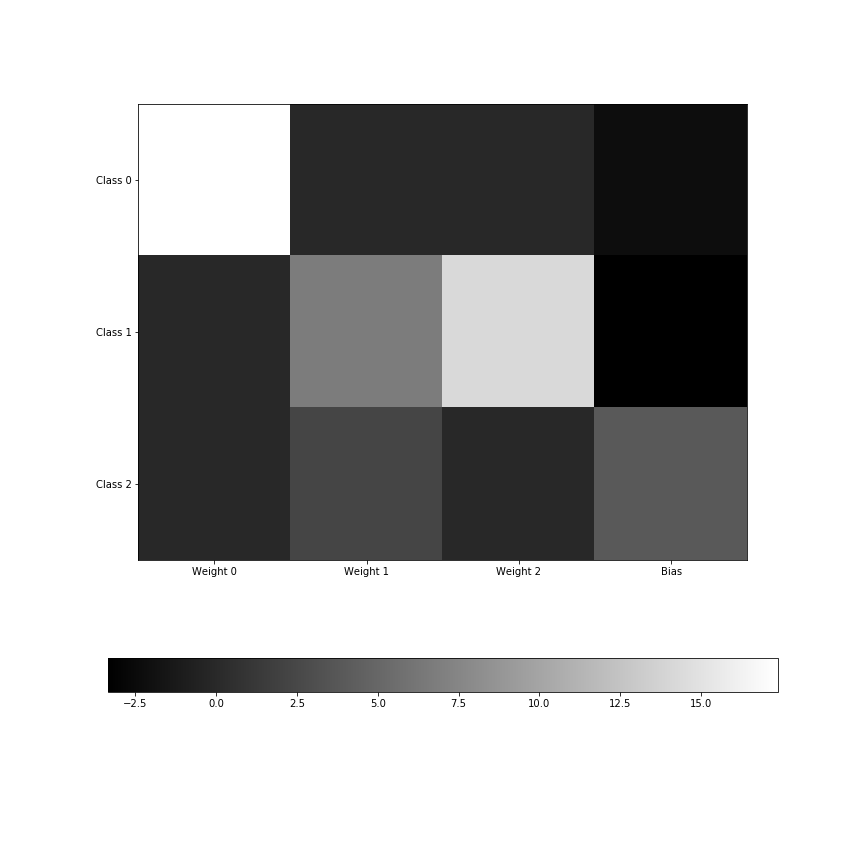
\includegraphics[width=0.23\textwidth]{figures/raman_sim_3_encode_layer_3_finetune_13.png}
\end{figure}


\begin{figure}
  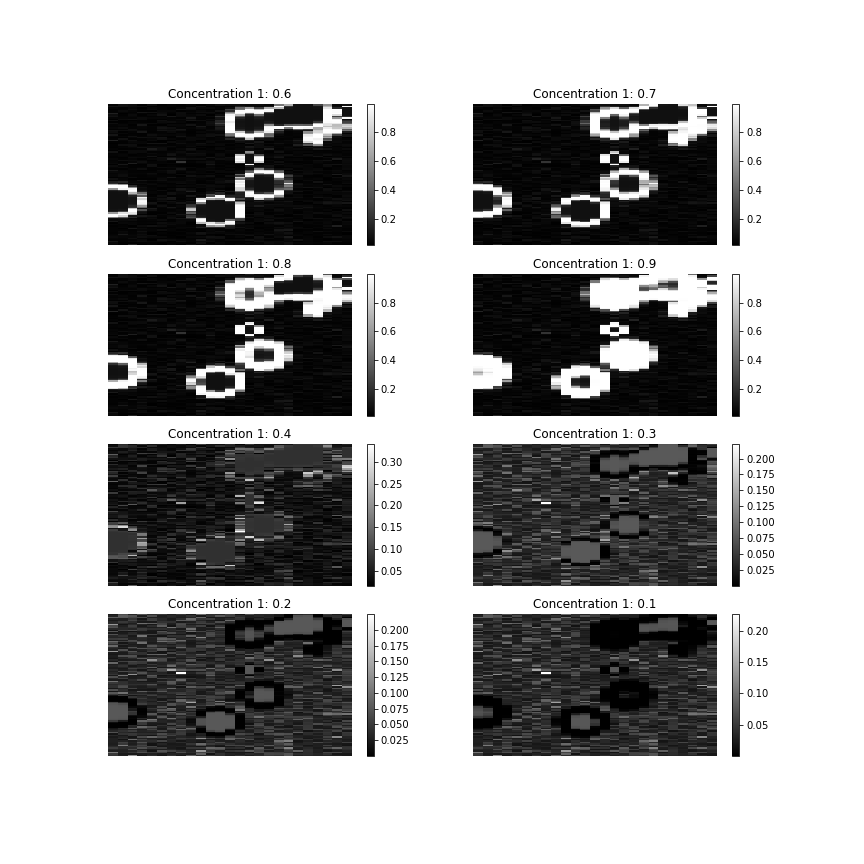
\includegraphics[width=0.30\linewidth]{figures/prop_substance_1_im.png}
  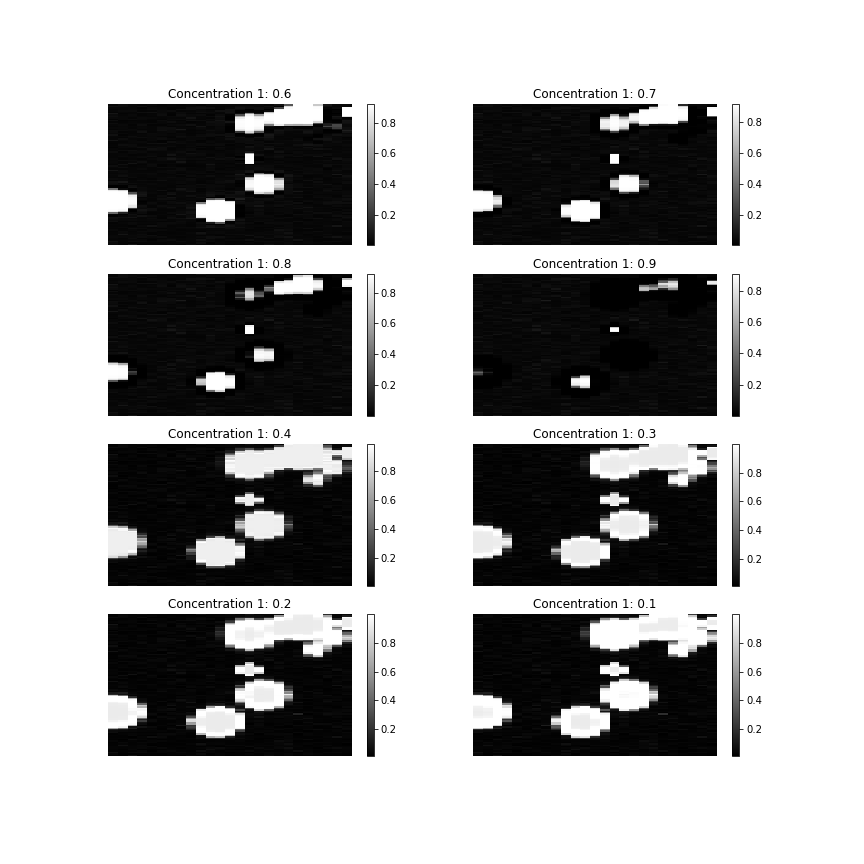
\includegraphics[width=0.30\linewidth]{figures/prop_substance_2_im.png}
  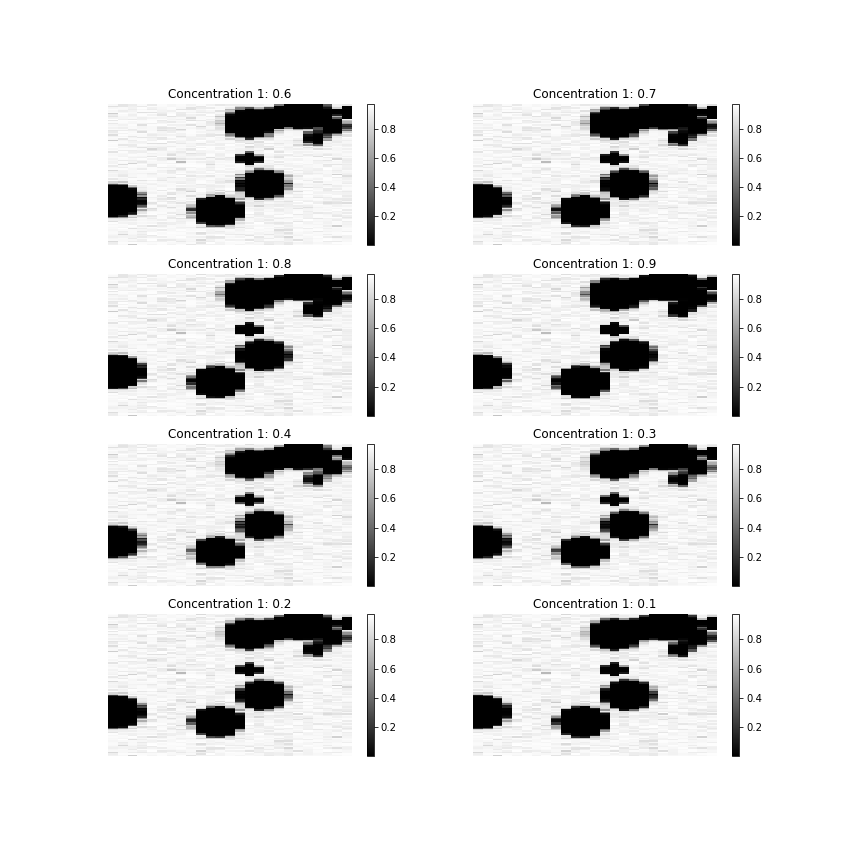
\includegraphics[width=0.30\linewidth]{figures/prop_substance_3_im.png}
\end{figure}



\begin{figure}
  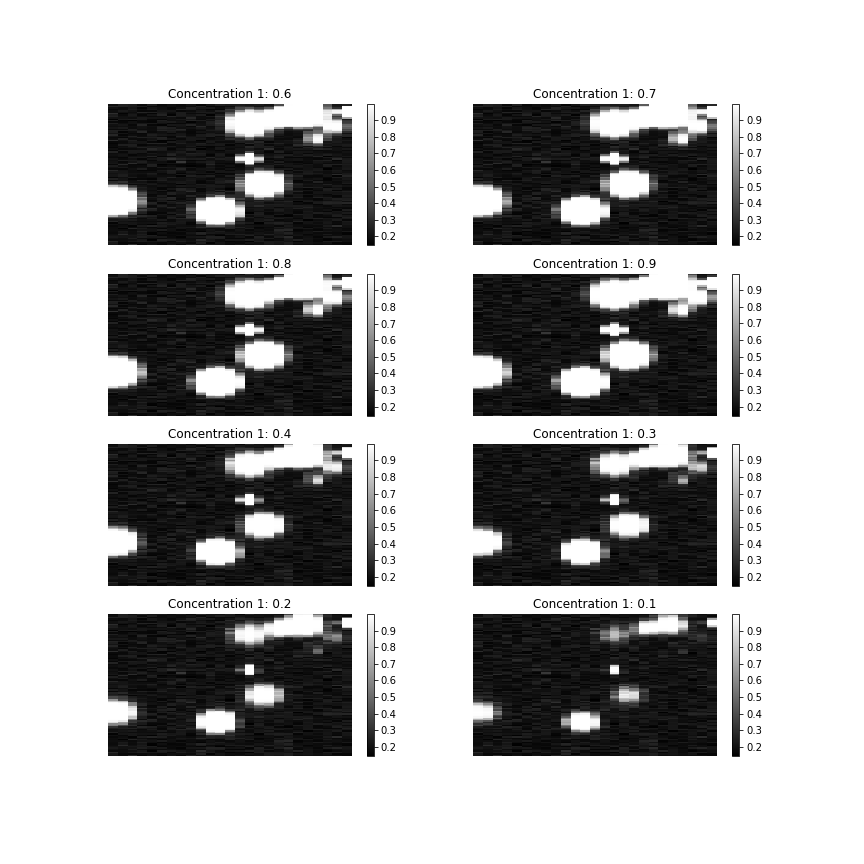
\includegraphics[width=0.30\linewidth]{figures/sigmoid_1_im.png}
  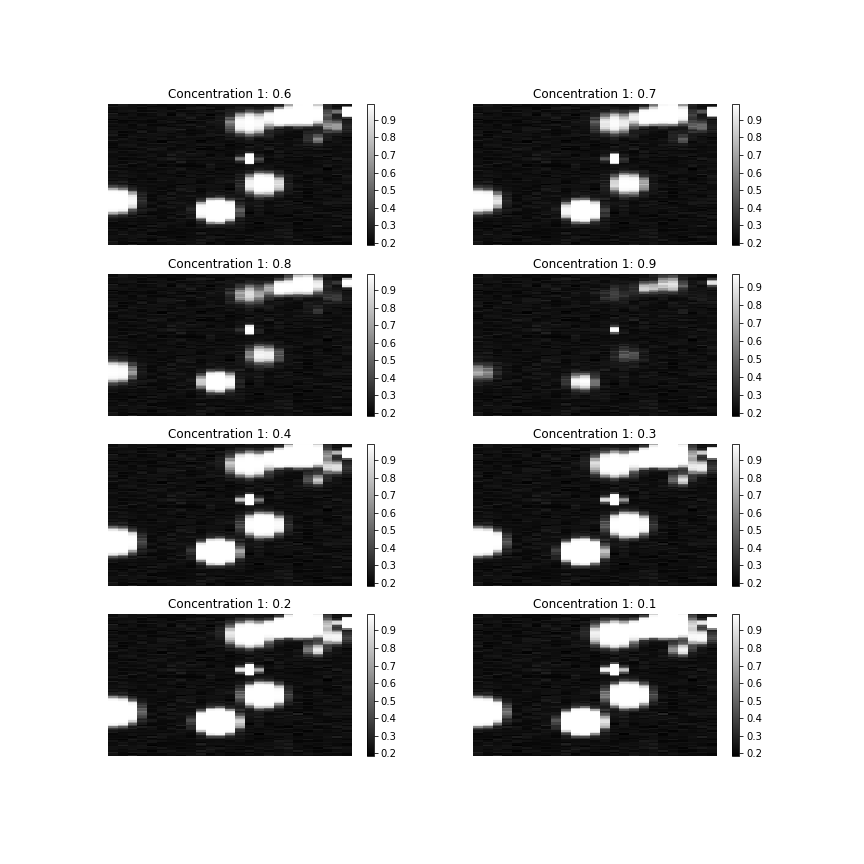
\includegraphics[width=0.30\linewidth]{figures/sigmoid_2_im.png}
  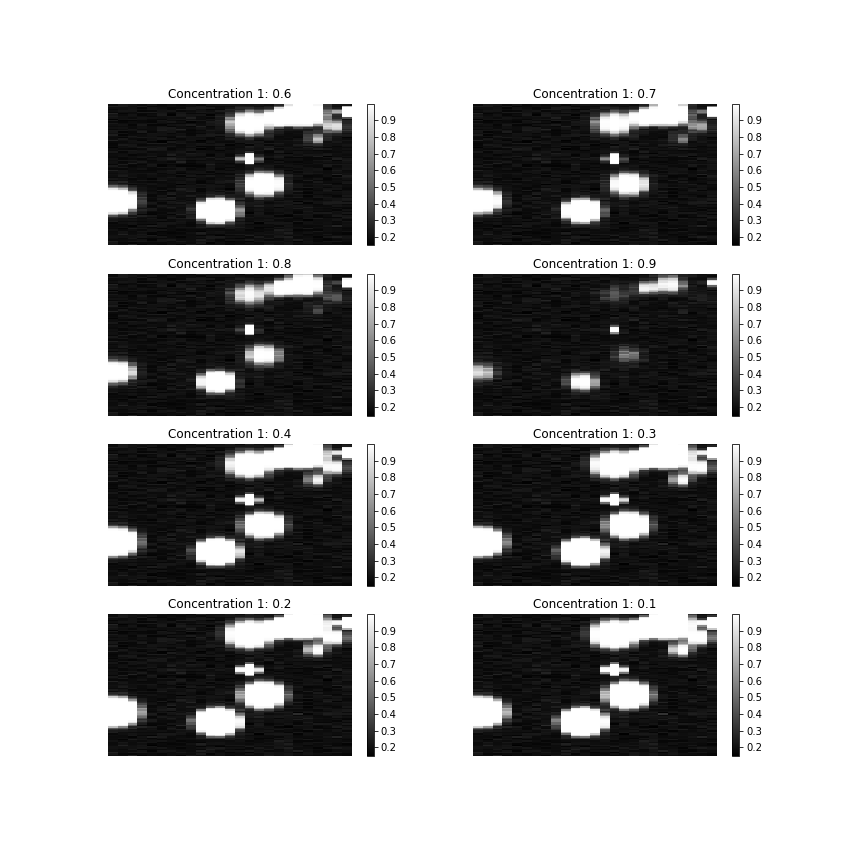
\includegraphics[width=0.30\linewidth]{figures/sigmoid_3_im.png}
\end{figure}



Classifier results


\begin{figure}
  
  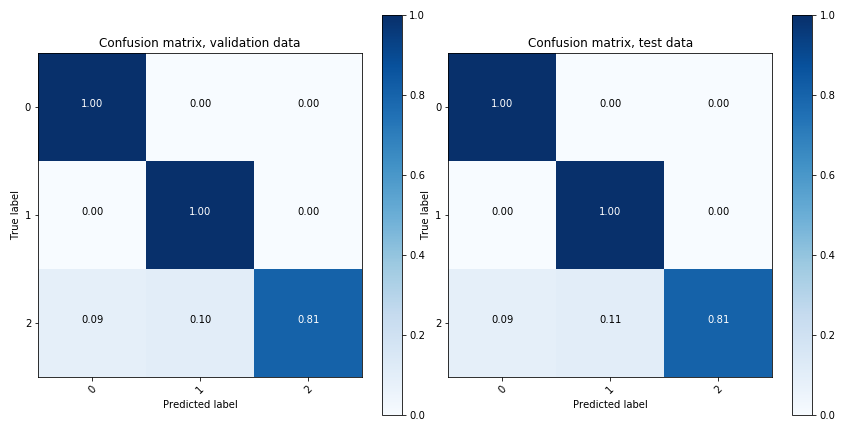
\includegraphics[width=0.5\textwidth]{figures/raman_sim_3_conf_matrix13.png}

\end{figure}

\section{Discussion}
\label{sec:discussion}


\begin{figure}
  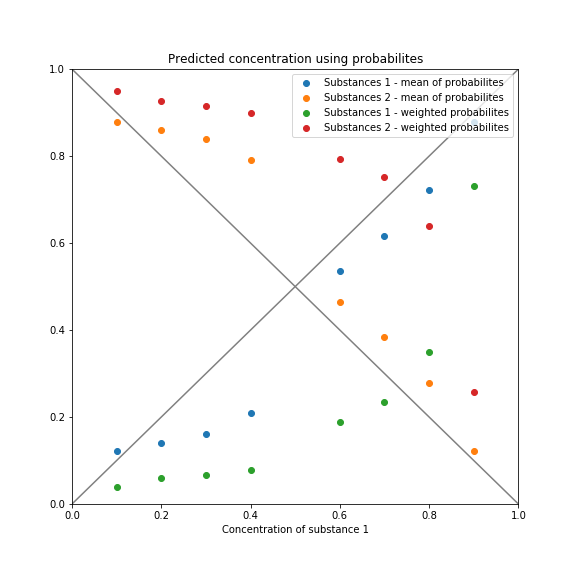
\includegraphics[width=0.23\textwidth]{figures/DNN_pred_conc_prob.png}
  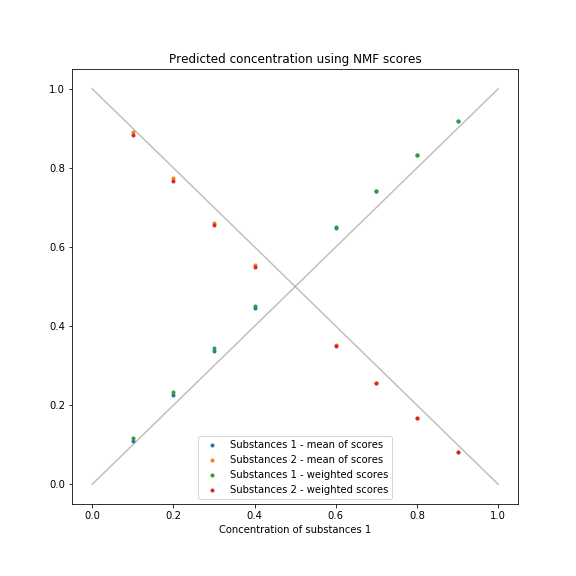
\includegraphics[width=0.23\textwidth]{figures/nmf_pred_conc.png}
\end{figure}

Comparison with NMF

\section{Conclusion}
\label{ssec:conclusion}


% Below is an example of how to insert images. Delete the ``\vspace'' line,
% uncomment the preceding line ``\centerline...'' and replace ``imageX.ps''
% with a suitable PostScript file name.

% To start a new column (but not a new page) and help balance the last-page
% column length use \vfill\pagebreak.
% -------------------------------------------------------------------------
\vfill
\pagebreak



\section{REFERENCES}
\label{sec:ref}

List and number all bibliographical references at the end of the paper.  The references can be numbered in alphabetic order or in order of appearance in the document.  When referring to them in the text, type the corresponding reference number in square brackets as shown at the end of this sentence .

% References should be produced using the bibtex program from suitable
% BiBTeX files (here: strings, refs, manuals). The IEEEbib.bst bibliography
% style file from IEEE produces unsorted bibliography list.
% -------------------------------------------------------------------------
\bibliographystyle{IEEEbib}
\bibliography{mendeley}

\end{document}
